\section{Systematics Uncertainties}
\label{sec:SystUncert}

%----
The uncertainties considered in the following may affect the overall normalization of the process, the shapes of the templates, or both. All the experimental uncertainties considered, with the exception of that in the luminosity, affect both normalization and shape in all the simulated samples. Uncertainties related to the modeling of the signal and background affect both normalization and shape, with the exception of cross-section and $t\bar{t}$ modeling uncertainties. The former only affects the normalization of the considered sample, while the latter only affects the shape of $t\bar{t}$ samples. Nevertheless, the normalization uncertainties modify the relative fractions of the different samples, leading to a shape uncertainty in the final distributions.

A single independent nuisance parameter is assigned to each source of systematic uncertainty in the statistical analysis. Some of the systematic uncertainties, in particular most of the experimental ones, are decomposed into several independent sources, as specified in the following. Each individual source then has a correlated effect across all analysis regions and signal and background samples. Table \ref{tb:SystSources} presents a list of all systematic uncertainties considered and indicates for each category the number of independent components and whether they affect the normalization of shape.

\begin{longtable}[hp]{lcc}
    \hline\hline
    \textbf{Systematic uncertainty} & \textbf{Type} & \textbf{Components}\\
    \endfirsthead

    % \hline\hline
    % \textbf{Systematic uncertainty} & \textbf{Type} & \textbf{Components}\\
    \endhead

    \endfoot
    \endlastfoot
    
    \hline
    \textbf{Experimental uncertainties} & &\\
    \hline
    \multicolumn{1}{l}{Luminosity}       &  N & 1\\
    \multicolumn{1}{l}{Pileup modeling} & SN & 1\\
    \hline
    \textit{Physics objects} & &\\
    \multicolumn{1}{l}{Electrons}                     & SN &  7\\
    \multicolumn{1}{l}{Muons}                         & SN & 15\\
    \multicolumn{1}{l}{Small-R jet energy scale}      & SN & 31\\
    \multicolumn{1}{l}{Small-R jet energy resolution} & SN &  9\\
    \multicolumn{1}{l}{Small-R jet mass scale}        & SN &  8\\
    \multicolumn{1}{l}{Large-R jet energy scale}      & SN & 24\\
    \multicolumn{1}{l}{Large-R jet energy resolution} & SN & 12\\
    \multicolumn{1}{l}{Large-R jet mass scale}        & SN & 18\\
    \multicolumn{1}{l}{Large-R jet mass resolution}   & SN & 10\\
    \multicolumn{1}{l}{Jet vertex tagger}             & SN &  1\\
    %\multicolumn{1}{l}{$E_\text{T}^\text{miss}$}      & SN &  3\\
    \hline
    \textit{$b$-tagging} & &\\
    \multicolumn{1}{l}{Efficiency}                            & SN &  9\\
    \multicolumn{1}{l}{Mis-tag rate (c)}                      & SN &  4\\
    \multicolumn{1}{l}{Mis-tag rate (light)}                  & SN &  4\\
    \multicolumn{1}{l}{$p_\text{T}$ extrapolation efficiency} & SN &  2\\
    \hline
    \textit{top-tagging} & &\\
    \multicolumn{1}{l}{Signal efficiency}                            & SN &  9\\
    \multicolumn{1}{l}{$p_\text{T}$ extrapolation signal efficiency} & SN &  1\\
    \multicolumn{1}{l}{background efficiency}                        & SN &  5\\
    \multicolumn{1}{l}{inefficiency}                                 & SN &  3\\
    \hline
    \textbf{Signal and background modeling} & &\\
    \hline
    \textit{Signal} & &\\
    \multicolumn{1}{l}{PDF variations} & SN & 30\\
    \multicolumn{1}{l}{Scales}         & SN &  2\\
    \hline
    \textit{$t\bar{t}$ background} & &\\
    \multicolumn{1}{l}{PDF variations}                                        & SN                & 90\\
    \multicolumn{1}{l}{$t\bar{t}+\text{HF}$ normalization}                    & N (free-floating) &  1\\
    \multicolumn{1}{l}{$t\bar{t}+\text{light}$ normalization}                 & N (free-floating) &  1\\
    \multicolumn{1}{l}{$t\bar{t}+\text{light}$ modeling}                      & S                 &  6\\
    \multicolumn{1}{l}{$t\bar{t}+\geq1c$ modeling}                            & S                 &  6\\
    \multicolumn{1}{l}{$t\bar{t}+\geq1b$ modeling}                            & S                 &  7\\
    \multicolumn{1}{l}{$t\bar{t}+\text{jets}$ reweighting}                    & SN                &  1\\
    \multicolumn{1}{l}{$t\bar{t}+\geq1b$ fraction}                            & N                 &  1\\
    \hline
    \textit{Other backgrounds} & &\\
    \multicolumn{1}{l}{$t\bar{t}W$ cross-section}        & N  & 2\\
    \multicolumn{1}{l}{$t\bar{t}Z$ cross-section}        & N  & 2\\
    \multicolumn{1}{l}{$t\bar{t}W$ modeling}            & SN & 1\\
    \multicolumn{1}{l}{$t\bar{t}Z$ modeling}            & SN & 1\\
    \multicolumn{1}{l}{Single top cross-section}         & N  & 3\\
    \multicolumn{1}{l}{Single top modeling}             & SN & 6\\
    \multicolumn{1}{l}{W+jets normalization}             & N  & 3\\
    \multicolumn{1}{l}{Z+jets normalization}             & N  & 1\\
    \multicolumn{1}{l}{Diboson normalization}            & N  & 1\\
    \multicolumn{1}{l}{$t\bar{t}t\bar{t}$ cross-section} & N  & 3\\
    \hline\hline
    \hline

    \caption{List of systematic uncertainties included in the analysis. Each "S" and "N" of type means that the systematic source is considered the "Shape" and "Normalization" effect, respectively. When the type of systematic source is "SN", both "Shape" and "Normalization" effects are considered.}\\
    \label{tb:SystSources}\\
\end{longtable}

\subsection{Luminosity and pile-up modeling}
\label{subsec:SystOfLumiAndPU}

\subsubsection{Luminosity}
\label{subsec:SystOfLumi}
The uncertainty on the integrated luminosity for the full Run-2 dataset is 1.7\% \cite{ATLAS-CONF-2019-021}, obtained using LUCID-2 detector \cite{G.Avoni-2018} for the primary luminosity measurement.

\subsubsection{Pile-up modeling}
\label{subsec:SystOfPileupModelling}
A variation in the pile-up reweighting of the simulated events is included to cover the uncertainties in the ratio of the predicted and measured inelastic cross-sections in the fiducial volume defined by $M_{X}>13$ GeV, where $M_{X}$ is the mass of the hadronic system \cite{STDM-2015-05}

\subsection{Reconstructed objects}
\label{subsec:SystOfRecoObjs}
\subsubsection{Charged leptons}
\label{subsec:SystOfLep}
Uncertainties associated with charged leptons arise from the trigger selection, the object reconstruction, identification and isolation criteria, as well as the lepton momentum scale and resolution. The reconstruction, identification, and isolation efficiency of electrons and muons, as well as the efficiency of the trigger used to record the events, differ slightly between data and simulation, which is compensated for by dedicated scale factors (SFs). Efficiency SFs are measured using tag-and-probe techniques on $Z{\rightarrow}l^{+}l^{-}$ data and simulated samples \cite{PERF-2015-10,PERF-2017-01}, and are applied to the simulation to correct for the differences. The effect of these SFs as well as of their uncertainties are propagated as corrections to the MC event weight. In total, four independent components are considered for electrons and ten for muons.

\vskip.2\baselineskip

Additional sources of uncertainty originate from the corrections applied to adjust the lepton momentum scale and resolution in the simulation to match those in data, measured using reconstructed distributions of the $Z{\rightarrow}l^{+}l^{-}$ and $J/{\psi}{\rightarrow}l^{+}l^{-}$ masses, as well as the $E/p$ ratio measured in $W{\rightarrow}e{\nu}$ events, where $E$ and $p$ are the electron energy and momentum measured by the calorimeter and the tracker, respectively \cite{PERF-2015-10,EGAM-2018-01}. To evaluate the effect of momentum scale uncertainties, the event selection is redone with the lepton energy or momentum varied by $\pm{1{\sigma}}$. For the momentum resolution uncertainties, the event selection is redone by smearing the lepton energy or momentum. In total, three independent components are considered for electrons and five for muons.

\subsubsection{Small-$R$ jets, Large-$R$ jets}
\label{subsec:SystOfLep}
Uncertainties associated with jets arise from the efficiency of pile-up rejection by the JVT, from the jet energy scale (JES) and resolution (JER), from the jet mass scale (JMS) and resolution (JMR), and from $b$- and top-tagging.

\begin{description}
  %--- JVT
  \item[Jet vertex tagging:] \mbox{}\\
    Scale factors are applied to correct discrepancies between data and MC for JVT efficiencies. These SFs are estimated using $Z{\rightarrow}{\mu}^{+}{\mu}^{-}$ with tag-and-probe techniques similar to those in Ref.\cite{PERF-2014-03}, and the effect of these SFs as well as of their uncertainties are propagated as corrections to the MC event weight.

  %--- Small-R jet (JES, JER, JMS)
  \item[Small-$R$ jet:] \mbox{}\\
    The \textit{R4\_CategoryReduction\_FullJER.config} jet uncertainties configuration is used. The JES and its uncertainty for small-$R$ jets are derived by combining information from test-beam data, LHC collision data and simulation \cite{PERF-2016-04}. The uncertainties from these measurements are factorized into several independent sources. Additional uncertainties are considered, related to jet flavor (using the conservative default value of $50\pm{50}$\% for the quark/gluon fraction for all MC samples), pile-up corrections, $\eta$ dependence, high-$p_\text{T}$ jets, and differences between full and fast simulation, yielding a total of 31 independence sources.
    \vskip.1\baselineskip
    The JER was measured in Run-2 data and simulation as a function of jet $p_\text{T}$ and rapidity using dijet events, using a similar method as that in Ref.~\cite{PERF-2014-02}. The combined uncertainty is propagated by smearing the jet $p_\text{T}$ in MC, yielding to nine independent sources.
    \vskip.1\baselineskip
    The JMS uncertainties for small-$R$ jets are derived using the RTrk uncertainties that compare the ratio of the jet mass for calorimeter jets to the jet mass of track-based jets in data and MC simulation \cite{JETM-2018-02}. The six NPs are provided, which are related to baseline, modeling, tracking, and total statistics. The technique takes advantage of two independent measures of the jet's mass (in the calorimeter and using the ID), however, this assumption breaks in the care of particle flow jets which uses both calorimeter and tracking information. For PFlow jets, the uncertainties derived for EMTopo jets are used and two additional uncertainties are provided. These uncertainties are derived by comparing the jet mass of EMTopo and PFlow jets in data and MC. Two NPs are provided similarly to the Rtrk uncertainties related to baseline and modeling. The JMS uncertainties are intentionally derived after the application of the JES and JER smearing. This is different compared to large-$R$ jets where no nominal JER smearing is applied. The JES corrects the overall energy scale, which impacts the mass as it is applied to the full four-vector. The JMS correction and uncertainties are then a residual correction accounting for the distribution of energy within the jet. For this reason, the JES and JMS uncertainties are to first order uncorrelated effects. 

  %--- Large-R jet (JES, JER, JMS, JMR)
  \item[Large-$R$ jet:] \mbox{}\\
    The \textit{R10\_CategoryJES\_FullJER\_FullJMS.config} jet uncertainties configuration is used for JES, JER, and JMS variation. JES uncertainties for large-$R$ jets are derived using a similar approach as for small-$R$ jets \cite{JETM-2018-02}. The correlation between these two objects is taken into account in uncertainty evaluation. Additional uncertainties related to a topology of an event are included.
    \vskip.1\baselineskip
    The JER uncertainties for large-$R$ jets are derived in the same way as the small-$R$ jets uncertainties. The dijet balance asymmetry is used to evaluate the JER, which is sufficient to cover the fully supported kinematic regime for large-$R$ jet usage. The nominal data/MC difference is found to be consistent with 1 within uncertainty. For this reason, no nominal JER smearing is applied. Instead, the nominal data/MC difference from 1 is taken as an additional uncertainty on top of the uncertainties related to limited statistics, detector effects, or modeling. The FullJER model with 12 NPs is used. Both data and MC events are smeared to cover properly the correlations between jets in different regions of the detector.
    \vskip.1\baselineskip
    The JMS uncertainties for large-$R$ jets are derived from the forward folding technique (FF) in the limited region of $200~\text{GeV}<p_\text{T}<1000~\text{GeV}$ around the $W$ and top mass peaks \cite{JETM-2018-02,ATLAS-CONF-2020-022}. The Rtrk technique is used to extend this region to $200~\text{GeV}<p_\text{T}<3000~\text{GeV}$, $m<600~\text{GeV}$ and $|\eta|<2.0$. The forward folding method is used to fit the $W$ and top mass peaks in $t\bar{t}$ semileptonic events. The Rtrk method uses the double ratio of data/MC for calorimeter-only quantities and track-only quantities. This technique can cover a wider range in $p_\text{T}$, $\eta$, and mass. However, the forward folding technique is more precise in the lower $p_\text{T}$ region and the mass around the top and $W$ masses. The uncertainties from the two approaches are combined and fitted as a function $p_\text{T}$ in a given mass bin. Interpolation between mass bins is used to provide smooth uncertainties. The full set of JMS NPs is used in the analysis in order to allow possible combinations with other measurements. The NPs are related to limited statistics of measurements, detector effects, modeling, and selections. In addition, uncertainties related to interpolation between mass bins and uncertainties related to a difference between QCD and hadronic decay jet mass response are included.
    \vskip.1\baselineskip
    Measurements of the JMR in the $t\bar{t}$ semileptonic events are also used to constrain the JMR uncertainties by using the forward folding method \cite{JETM-2018-02, ATLAS-CONF-2020-022}. Measurements are performed in two mass regions to cover $W$ boson and top quark mass peaks. The $W$ boson mass peak is fitted in a region of $50~\text{GeV}<m_{\text{jet}}<120~\text{GeV}$ and $200~\text{GeV}<p_{\text{T,jet}}<350~\text{GeV}$. The top mass peak is fitted in a region of $120~\text{GeV}<m_{\text{jet}}<300~\text{GeV}$ and $350~\text{GeV}<p_{\text{T,jet}}<1000~\text{GeV}$. Relative JMR uncertainty of 20\% is used outside these regions. FullJMR uncertainty model with 10 nuisance parameters is used to cover uncertainties related to the measurement of JMR using the FF method, interpolation between bins, and the comparison between different MC models for events outside the two regions. This measurement is within the top mass interval. However, $p_{\text{T,jet}}$ exceeds the $p_{\text{T}}$ range provided by the FF method.
    %The \textit{R10\_FullJMR\_COMB\_newBinning.config} jet uncertainties configuration is used for JMR variation.

  %--- b-tagging    
  \item[$b$-tagging:] \mbox{}\\
    $b$-tagging efficiencies in simulated samples are corrected to match efficiencies in data. Scale factors are derived as a function of $p_\text{T}$ for jets containing $b$-jets, $c$-jets and for jets containing neither $b$- nor $c$-hadrons (light-jets) separately, in dedicated calibration analysis. For $b$-jets efficiencies, $t\bar{t}$ events in the dilepton topology are used, exploiting the very pure sample of $b$-jets arising from the decays of the top quarks \cite{FTAG-2018-01}. For $c$-jet mistag rates, $t\bar{t}$ events in single-lepton topology are used, exploiting the $c$-jets from the hadronically decaying $W$ bosons, using techniques similar to those in Ref.~\cite{ATLAS-CONF-2018-001}. For light-jets mistag rates, the so-called negative-tag method similar to that in Ref.~\cite{ATLAS-CONF-2018-006} is used, but using $Z+\text{jets}$ events instead of di-jet events. In the three calibration analyses, a large number of uncertainty components are considered, and a principal component analysis is performed, yielding in 45, 20, and 20 eigenvariations, respectively, for $b$-, $c$, and light-jets, which are taken as uncorrelated sources of uncertainties. The number of these eigenvariations corresponds to the number of $p_\text{T}$ bins (9, 4, and 4, respectively, for $b$-, $c$- and light-jets). The calibration used in this analysis is stored in the following "CDI file":\\
    \textit{/cvmfs/atlas.cern.ch/repo/sw/database/GroupData/xAODBTaggingEfficiency/13TeV/2020-21-13TeV-MC16-CDI-2021-04-16\_v1.root}.

  %--- top-tagging    
  \item[Top-tagging:] \mbox{}\\
    Uncertainties related to the top-tagging calibration are provided for the signal and the background jets \cite{JETM-2018-03, ATL-PHYS-PUB-2020-017}. Jets are called signals if they pass contained top criteria. Otherwise, they are called background jets. Uncertainties for background jets are measured in two-phase spaces containing QCD multijet and gamma+jet processes. The signal jets uncertainties are measured in the boosted $t\bar{t}$ lepton+jets channel in the range of leading large-R jet $p_{\text{T}}\leq1$ TeV, because there are too few $t\bar{t}$ events to extract scale factors for $p_{\text{T}}\geq1$ TeV. Therefore, additional uncertainties are assigned to cover signal modeling effects and extrapolation beyond the phase spaces. These uncertainties were released as part of the consolidated large-$R$ jet uncertainties.
    
\end{description}

\subsection{Signal modeling}
\label{subsec:SystOfSigModelling}
\newcounter{num}
\setcounter{num}{2}
The $H^{+}$ and $W'$ signal uncertainty is modeled in two ways: by using the PDF uncertainties and through the variation of $\mu_{f}$ and $\mu_{r}$. The uncertainties from the modeling of the PDF, which is done with the NNPDF2.3 or NNPDF3.0 PDF set for datasets simulated, are made using a symmetrized Hessan set, PDF4LHC15\_nlo\_30, following the PDF4LHC recommendations for LHC Run \Roman{num} \cite{Butterworth:2015oua}. The signal scale uncertainty is modeled by varying $\mu_{f}$ and $\mu_{r}$ up (and down) by a factor of 2 (or 0.5).

\subsection{Background modeling}
\label{subsec:SystOfBkgModeling}

\subsubsection{$t\bar{t}$+jets}
\label{subsec:SystOfTtbar}

\begin{description}
  \item[$t\bar{t}+\text{heavy flavor classification}$] \mbox{}\\
    The $t\bar{t}+\text{jets}$ background is categorized according to the flavor of additional jets in the event, using the same procedure as described in Ref. \cite{HIGG-2017-04}. Generator-level particle jets are reconstructed from stable particles (mean lifetime ${\tau}>3{\times}10^{-11}$ seconds) using the anti-$k_t$ algorithm with a radius parameter $R=0.4$, and are required to have $p_\text{T}>15$ GeV and $|\eta|<2.5$. The flavor of a jet is determined by counting the number of $b$- or $c$-hadrons within ${\Delta}R<0.4$ of the jet axis. Jets matched to exactly one $b$-hadron, with $p_\text{T}$ above 5 GeV, are labeled single-$b$-jets, while those matched to two or more $b$-hadrons are labeled $b$-jets (with no $p_\text{T}$ requirement on the second hadron); single-$c$- and $c$-jets are defined analogously, only considering jets not already defined as single-$b$- or $b$-jets. Events that have at least one single-$b$- or $b$-jet, not counting heavy-flavor jets from top-quark or $W$-boson decays, are labeled as $t\bar{t}+{\geq}1b$; those with no single-$b$- or $b$-jet but at least one single-$c$- or $c$-jet are labeled as $t\bar{t}+{\geq}1c$. Finally, events not containing any heavy-flavor jets aside from those from top-quark or $W$-boson decays are labeled as $t\bar{t}+\text{light}$. This classification is used to define the background categories in the likelihood fit.
    
  \item[Systematic uncertainties] \mbox{}\\
    The systematic uncertainties affecting the $t\bar{t}+\text{jets}$ background modeling are summarized in Table \ref{tb:TtbarSystSources}. 
    % --- Normalisation and ttb fraction
    The normalization of $t\bar{t}+\text{light}$, $t\bar{t}+\geq1c$ and $t\bar{t}+\geq1b$ are allowed to vary freely in the fit. The normalization factors of $t\bar{t}+\geq1c$ and $t\bar{t}+\geq1b$ are estimated with a common parameter in the fit. However, since these distribution's shapes are different slightly from each other in the high BDT score region as shown in Figure \ref{fig:CompTtbarShapeInSR1}. Therefore, the uncertainty of the $t\bar{t}+\geq1b$ fraction to the whole of $t\bar{t}+\text{HF}$ can be a systematic source because it changes the whole template shape of $t\bar{t}+\geq1c$ and $t\bar{t}+\geq1b$. Referring to the post-fit results of the resolved analysis \cite{HDBS-2021-02}, the observed fraction ($R_{\text{ttb}}^{\text{Data}}$) differs from the expected one ($R_{\text{ttb}}^{\text{MC}}$) by about 12\% as follows:
    \begin{alignat}{1}
        R_{\text{ttb}}^{\text{MC}} = \frac{\text{N}_{\text{ttb}}^{\text{MC}}}{\text{N}_{\text{ttb}^{\text{MC}}} + \text{N}_{\text{ttc}}^{\text{MC}}} \sim 0.64,
        \quad R_{\text{ttb}}^{\text{Data}} = \frac{\text{N}_{\text{ttb}}^{\text{Data}}}{\text{N}_{\text{ttb}^{\text{Data}}} + \text{N}_{\text{ttc}}^{\text{Data}}} & \sim 0.72,
        \quad \frac{R_{\text{ttb}}^{\text{Data}}}{R_{\text{ttb}}^{\text{MC}}} \sim 0.88 \notag
    \end{alignat}
    In this analysis, the fraction uncertainty is assumed conservatively enough to be $\pm 50\%$, and an NP is introduced. The total amount of $t\Bar{t}+\text{HF}$ is kept the same after changing the fraction.
    
    \begin{figure}[H]
      \centering
      \subfloat[]{
        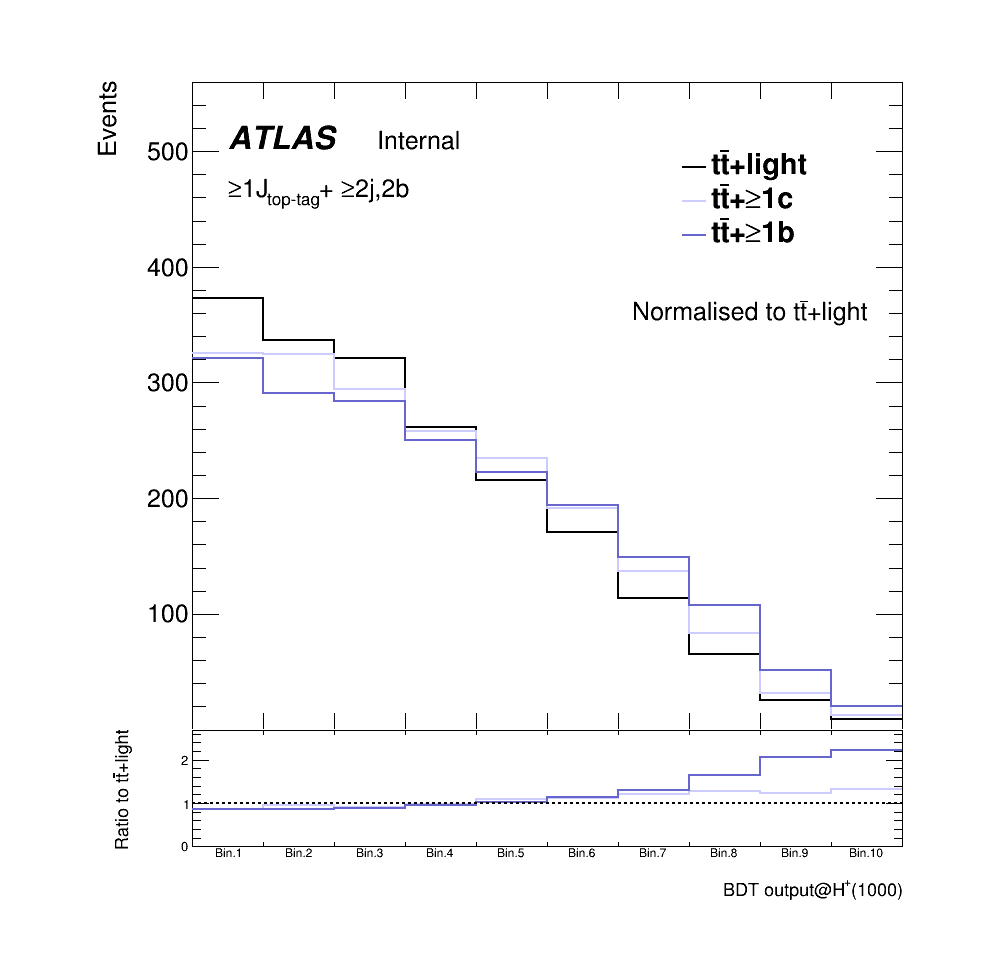
\includegraphics[width=0.45\textwidth]{images/Systematics/TTBarComparison_bdt_Hp1000_geq1tgeq2j2b.png}
        \label{fig:CompTtbarShapeInSR1_bdtHp1000}
      }
      \subfloat[]{
        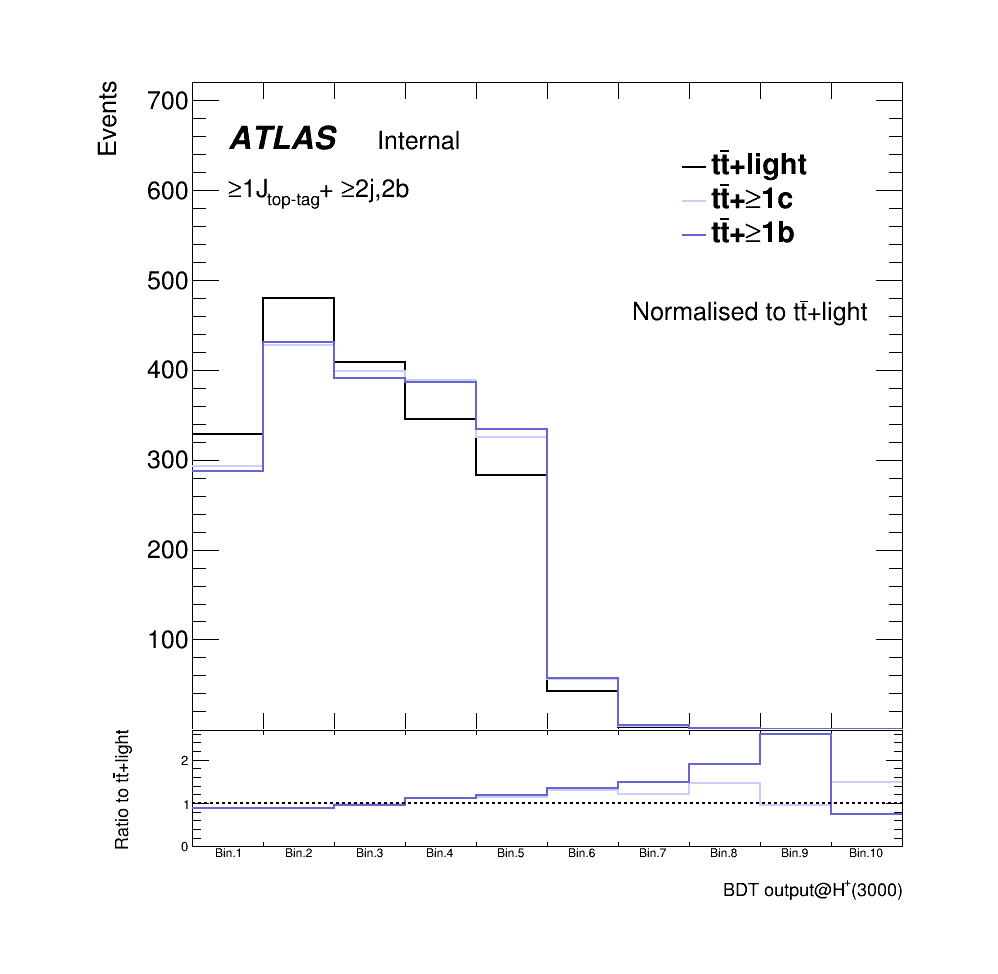
\includegraphics[width=0.45\textwidth]{images/Systematics/TTBarComparison_bdt_Hp3000_geq1tgeq2j2b.png}
        \label{fig:CompTtbarShapeInSR1_bdtHp3000}
      }
      \caption{Comparison of the shape of BDT distributions in the SR1 among $t\Bar{t}+\text{jets}$ events, where (a) is BDT output trained using 1000 GeV $H^{+}$ samples, and (b) is the one trained using 3000 GeV. $t\bar{t}+\geq1c$ and $t\bar{t}+\geq1b$ distributions are normalised to the distribution of $t\bar{t}+\text{light}$. And the ratios to $t\bar{t}+\text{light}$ distribution are shown at the bottom.}
      \label{fig:CompTtbarShapeInSR1}
    \end{figure}

    % --- Normalisation and ttb fraction
    Besides normalization, the $t\bar{t}+\text{light}$, $t\bar{t}+\geq1c$ and $t\bar{t}+\geq1b$ processes are affected by different types of uncertainties: $t\bar{t}+\text{light}$ has additional diagrams and profits from relatively precise measurements in data; $t\bar{t}+\geq1c$ and $t\bar{t}+\geq1b$ can have similar or different diagrams depending on the flavor scheme used for the PDF, and different mass of the $c$- and $b$-quark contribute to additional differences between these two processes. For these reasons, all uncertainties in the $t\bar{t}+\text{jets}$ background modeling are assigned independent nuisance parameters for the $t\bar{t}+\text{light}$, $t\bar{t}+\geq1c$ and $t\bar{t}+\geq1b$ processes.

    % --- Reweighting
    Systematic uncertainties on the reweighting are extracted according to the reweighting functions derived in Section \ref{subsec:ReweightingTechnique}. The differences between the BDT output distribution reweighted with the nominal reweighting function and the one reweighted with ${\pm}1{\sigma}$ functions are included in the fit for each $t\bar{t}+\text{jets}$ as an NP.
    
    Systematic uncertainties on the acceptance and shapes are extracted from the comparison between the nominal and different MC samples and settings. For ISR and FSR the settings of the nominal Powheg+Pythia sample are varied, resulting in different event weights; the uncertainty due to ISR is estimated by changing $\mu_{r}$ and $\mu_{f}$ in the ME and $\alpha_{S}^{\text{ISR}}$ in the PS, while the uncertainty due to FSR is estimated by changing $\alpha_{S}^{\text{FSR}}$ in the PS. For the ISR, the amount of radiation is increased (decreased) by scaling $\mu_{r}$ and $\mu_{f}$ by a factor 0.5 (2.0) and by using the $\text{Var3cUp (Var3cDown)}$ variation from the A14 tune \cite{ATL-PHYS-PUB-2014-021}, corresponding to $\alpha_{S}^{\text{ISR}}=0.140(0.115)$ instead of the nominal $\alpha_{S}^{\text{ISR}}=0.127$. For the FSR, the amount of radiation is increased (decreased) varying $\mu_{r}$ for QCD emission in the FSR by a factor of 0.5 (2.0), corresponding to $\alpha_{S}^{\text{FSR}}=0.1423(0.1147)$ instead of the nominal $\alpha_{S}^{\text{FSR}}=0.127$. The nominal Powheg+Pythia sample is compared to the Powheg+Herwig sample to access the effect of the PS and hadronization models, and to the MG5\_aMC sample to access the effect of the NLO matching technique.

    %--- 4FS vs. 5FS for ttb
    The nominal prediction for the dominant $t\bar{t}+\geq1b$ background, based on the Powheg+Phytia $t\bar{t}$ (5FS) sample in which all the additional partons are produced by the PS, is compared to the alternative Powheg+Phythia $t\bar{t}$ (4FS) sample, in which the $b\bar{b}$ pair is generated in addition to the $t\bar{t}$ pair at the ME level at NLO in QCD. A uncertainty resulting from the comparison of the shape of the two models is included.

    %--- ttbar systematic sources table
    \begin{table}[H]
      \centering
      \begin{tabular*}{160mm}{@{\extracolsep{\fill}}llll}
        \hline\hline
        Uncertainty source & \multicolumn{2}{l}{Description} & Components\\
        \hline
        $t\bar{t}+\text{light}$ normalization   & \multicolumn{2}{l}{Free-floating}                                                               & $t\bar{t}+\text{light}$\\
        $t\bar{t}+\text{HF}$ normalization      & \multicolumn{2}{l}{Free-floating}                                                               & $t\bar{t}+\geq{1b}$ and $t\bar{t}+\geq{1c}$\\
        $t\bar{t}+\geq1b$ fraction              & \multicolumn{2}{l}{Fraction to the whole of $t\bar{t}+\text{HF}$}                               & $t\bar{t}+\geq{1b}$ and $t\bar{t}+\geq{1c}$\\
        $t\bar{t}+\text{jets}$ reweighting      & \multicolumn{2}{l}{Statistical uncertainties of weights}                                        & All $t\bar{t}+\text{jets}$\\
        $t\bar{t}+\geq1b$ flavor scheme         & \multicolumn{2}{l}{5FS vs 4FS}                                                                  & $t\bar{t}+\geq{1b}$\\
        \hline
        NLO matching              & MG5\_aMC+Pythia                        & vs. Powheg+Pythia & All \\
        PS \& hadronisation       & Powheg+Herwig                          & vs. Powheg+Pythia & All \\
        $\alpha_{S}^{\text{ISR}}$ & $Var3cUp$ ($Var3cDown$)                & in Powheg+Pythia  & All \\
        $\mu_{f}$                 & scaling by 0.5 (2.0)                   & in Powheg+Pythia  & All \\
        $\mu_{r}$                 & scaling by 0.5 (2.0)                   & in Powheg+Pythia  & All \\
        FSR                       & Varying $\alpha_{S}^{\text{FSR}}$ (PS) & in Powheg+Pythia  & All \\
        \hline\hline
      \end{tabular*}
      \caption{Summary of the sources if systematic uncertainty for $t\bar{t}+\text{jets}$ modeling. The systematic uncertainties listed in the second section of the table are evaluated in such a way to have no impact on the normalization of the three, $t\bar{t}+\text{light}$, $t\bar{t}+\geq1c$ and $t\bar{t}+\geq1b$ components in the phase-space selected in the analysis. The last column of the table indicates the $t\bar{t}+\text{jets}$ components to which a systematic uncertainty is assigned. All systematic uncertainty sources are treated as uncorrelated across the three components.}
      \label{tb:TtbarSystSources}
    \end{table}

    
\end{description}

%--- Sec. 5.4.2
\subsubsection{Other backgrounds}
\label{subsec:SystOfOtherBkg}
%--- ttH
The predicted $t\bar{t}H$ signal cross-section uncertainty is ${}^{+5.8\%}_{-9.2\%}\text{ }(\text{QCD scale})\pm{3.6\%}\text{ }(\text{PDF}+{\alpha}_{S})$ \cite{deFlorian:2016spz, R.Raitio-1979, W.Beenaller-2002, S.Dawson-2003, Y.Zhang-2014, S.Frixione-2015}. These two components are treated as uncorrelated in the fit. The effect of QCD scale and PDF variations on the shape of the distributions is found to be negligible. Uncertainties in the Higgs-boson branching fractions are also considered; these amount to 2.2\% for the $b\bar{b}$ decay mode \cite{deFlorian:2016spz}. Uncertainties associated to the modeling of $t\bar{t}H$ by the Powheg+Phythia sample are also considered, for a total of four independent components. The uncertainty due to ISR  is estimated by simultaneously changing $\mu_{f}$ and $\mu_{r}$ in the ME and ${\alpha}^{\text{ISR}}_{S}$ in the PS, while the uncertainty due to ISR is estimated by changing ${\alpha}^{\text{FSR}}_{S}$ in the PS. For the ISR and FSR, the amount of radiation is varied following the same procedure as for $t\bar{t}$. The nominal Powheg+Pythia sample is compared to the Powheg+Herwig sample to access the uncertainty due to PS and hadronization, and to the MG5\_aMC+Phythia sample for the uncertainty due to the NLO matching.

%--- single top
\vskip.2\baselineskip
A $\pm{5}$\% uncertainty is considered for the cross-sections of the three single-top production modes \cite{LHCTopWGsgtopXsec, Martin:2009iq, Martin:2009bu, Aliev:2010zk, Kant:2014oha}. Uncertainties associated with the PS and hadronisation model, and with the NLO matching scheme are evaluated by comparing, for each process, the nominal Powheg+Pythia sample to a sample produced using Powheg+Herwig and MG5\_aMC+Pythia, respectively. The uncertainty associated to the interference between $Wt$ and $t\bar{t}$ production at NLO \cite{Frixione:2008yi} is assessed by comparing the nominal Powheg+Pythia sample produced using the "diagram removal" scheme to an alternative sample produced with the same generator but using the "diagram subtraction" scheme.

%--- ttV
\vskip.2\baselineskip
The uncertainty of the $t\bar{t}V$ NLO cross-section prediction is 15\% \cite{LHCHXSWGTTH-twiki, J.M.Campbell-2012}, split into PDF and scale uncertainties as for $t\bar{t}H$. An additional $t\bar{t}V$ modeling uncertainty, related to the choice of PS and hadronisation model and NLO matching scheme is assessed by comparing the nominal MG5\_aMC+Pythia samples with alternative ones generated with Sherpa.

%--- small top background
\vskip.2\baselineskip
A total 50\% normalization uncertainty is considered for the 4 tops background, covering effects from varying $\mu_{f}$ and $\mu_{r}$, PDFs and $\alpha_{S}$ \cite{Alwall:2014hca, PmgTopProcesses-twiki}. The small backgrounds from $tZq$ and $tWH$ are each assigned cross-section uncertainties: $\pm{7.9}$\% and $\pm{0.9}$\% for $tZq$, accounting for $\mu_{f}$ and $\mu_{r}$ variations, and for PDFs, respectively, and $\pm{50}$\% for $tWZ$ \cite{Alwall:2014hca}.

%--- VV and V+jets
\vskip.2\baselineskip
An uncertainty of 40\% is assumed for the $W+\text{jets}$ cross-section, with an additional 30\% normalization uncertainty used for $W+\text{heavy-flavor jets}$, taken as uncorrelated between events with two and more than two heavy-flavor jets. These uncertainties are based on variations of the $\mu_{f}$ and $\mu_{r}$ and of the matching parameters in the Sherpa samples. An uncertainty of 35\% is then applied to the $Z+\text{jets}$ normalization, uncorrelated across jet bins, to account for both the variations of the scales and matching parameters in the Sherpa samples and the uncertainty in the extraction from data of the correction factor for the heavy-flavor component. Finally, a total 50\% normalization uncertainty in the diboson background is assumed, which includes uncertainties in the inclusive cross-section and additional jet production \cite{ATL-PHYS-PUB-2016-002}.